\section{Experimental Results}

    % Setup dell'esperimento (hardware, software, ecc) con foto
    % Parlare delle tre versioni disponibili (19 gennaio e ultima + differenze) 
    % Bordo nero - divisa in diverse funzioni (crop, enlarge, zoom) (19/01)
    % Bordo nero - unica funzione (26/01)
    % Tolto bordo nero - (ultima versione)
    % Comparison dei risultati in queste versioni (tempo di esecuzione, visione dell'immagine)
    % Discutere le differenze di zooming level in base alla grandezza del ritaglio (in pixel)
    % 
    \subsection{Experimental setup}
    The project has been carried out using a Jetson Nano [\ref{fig:jetson}], a small single-board computer with a quad-core ARM Cortex-A57 CPU and a Maxwell GPU. 
    The Jetson Nano is equipped with 4GB of RAM and an SDCard for the Operating System and data storage. The operating system used is Ubuntu 18.04.3 LTS and the CUDA version is 10.0.326. 

    \begin{figure}[h]
        \centering
        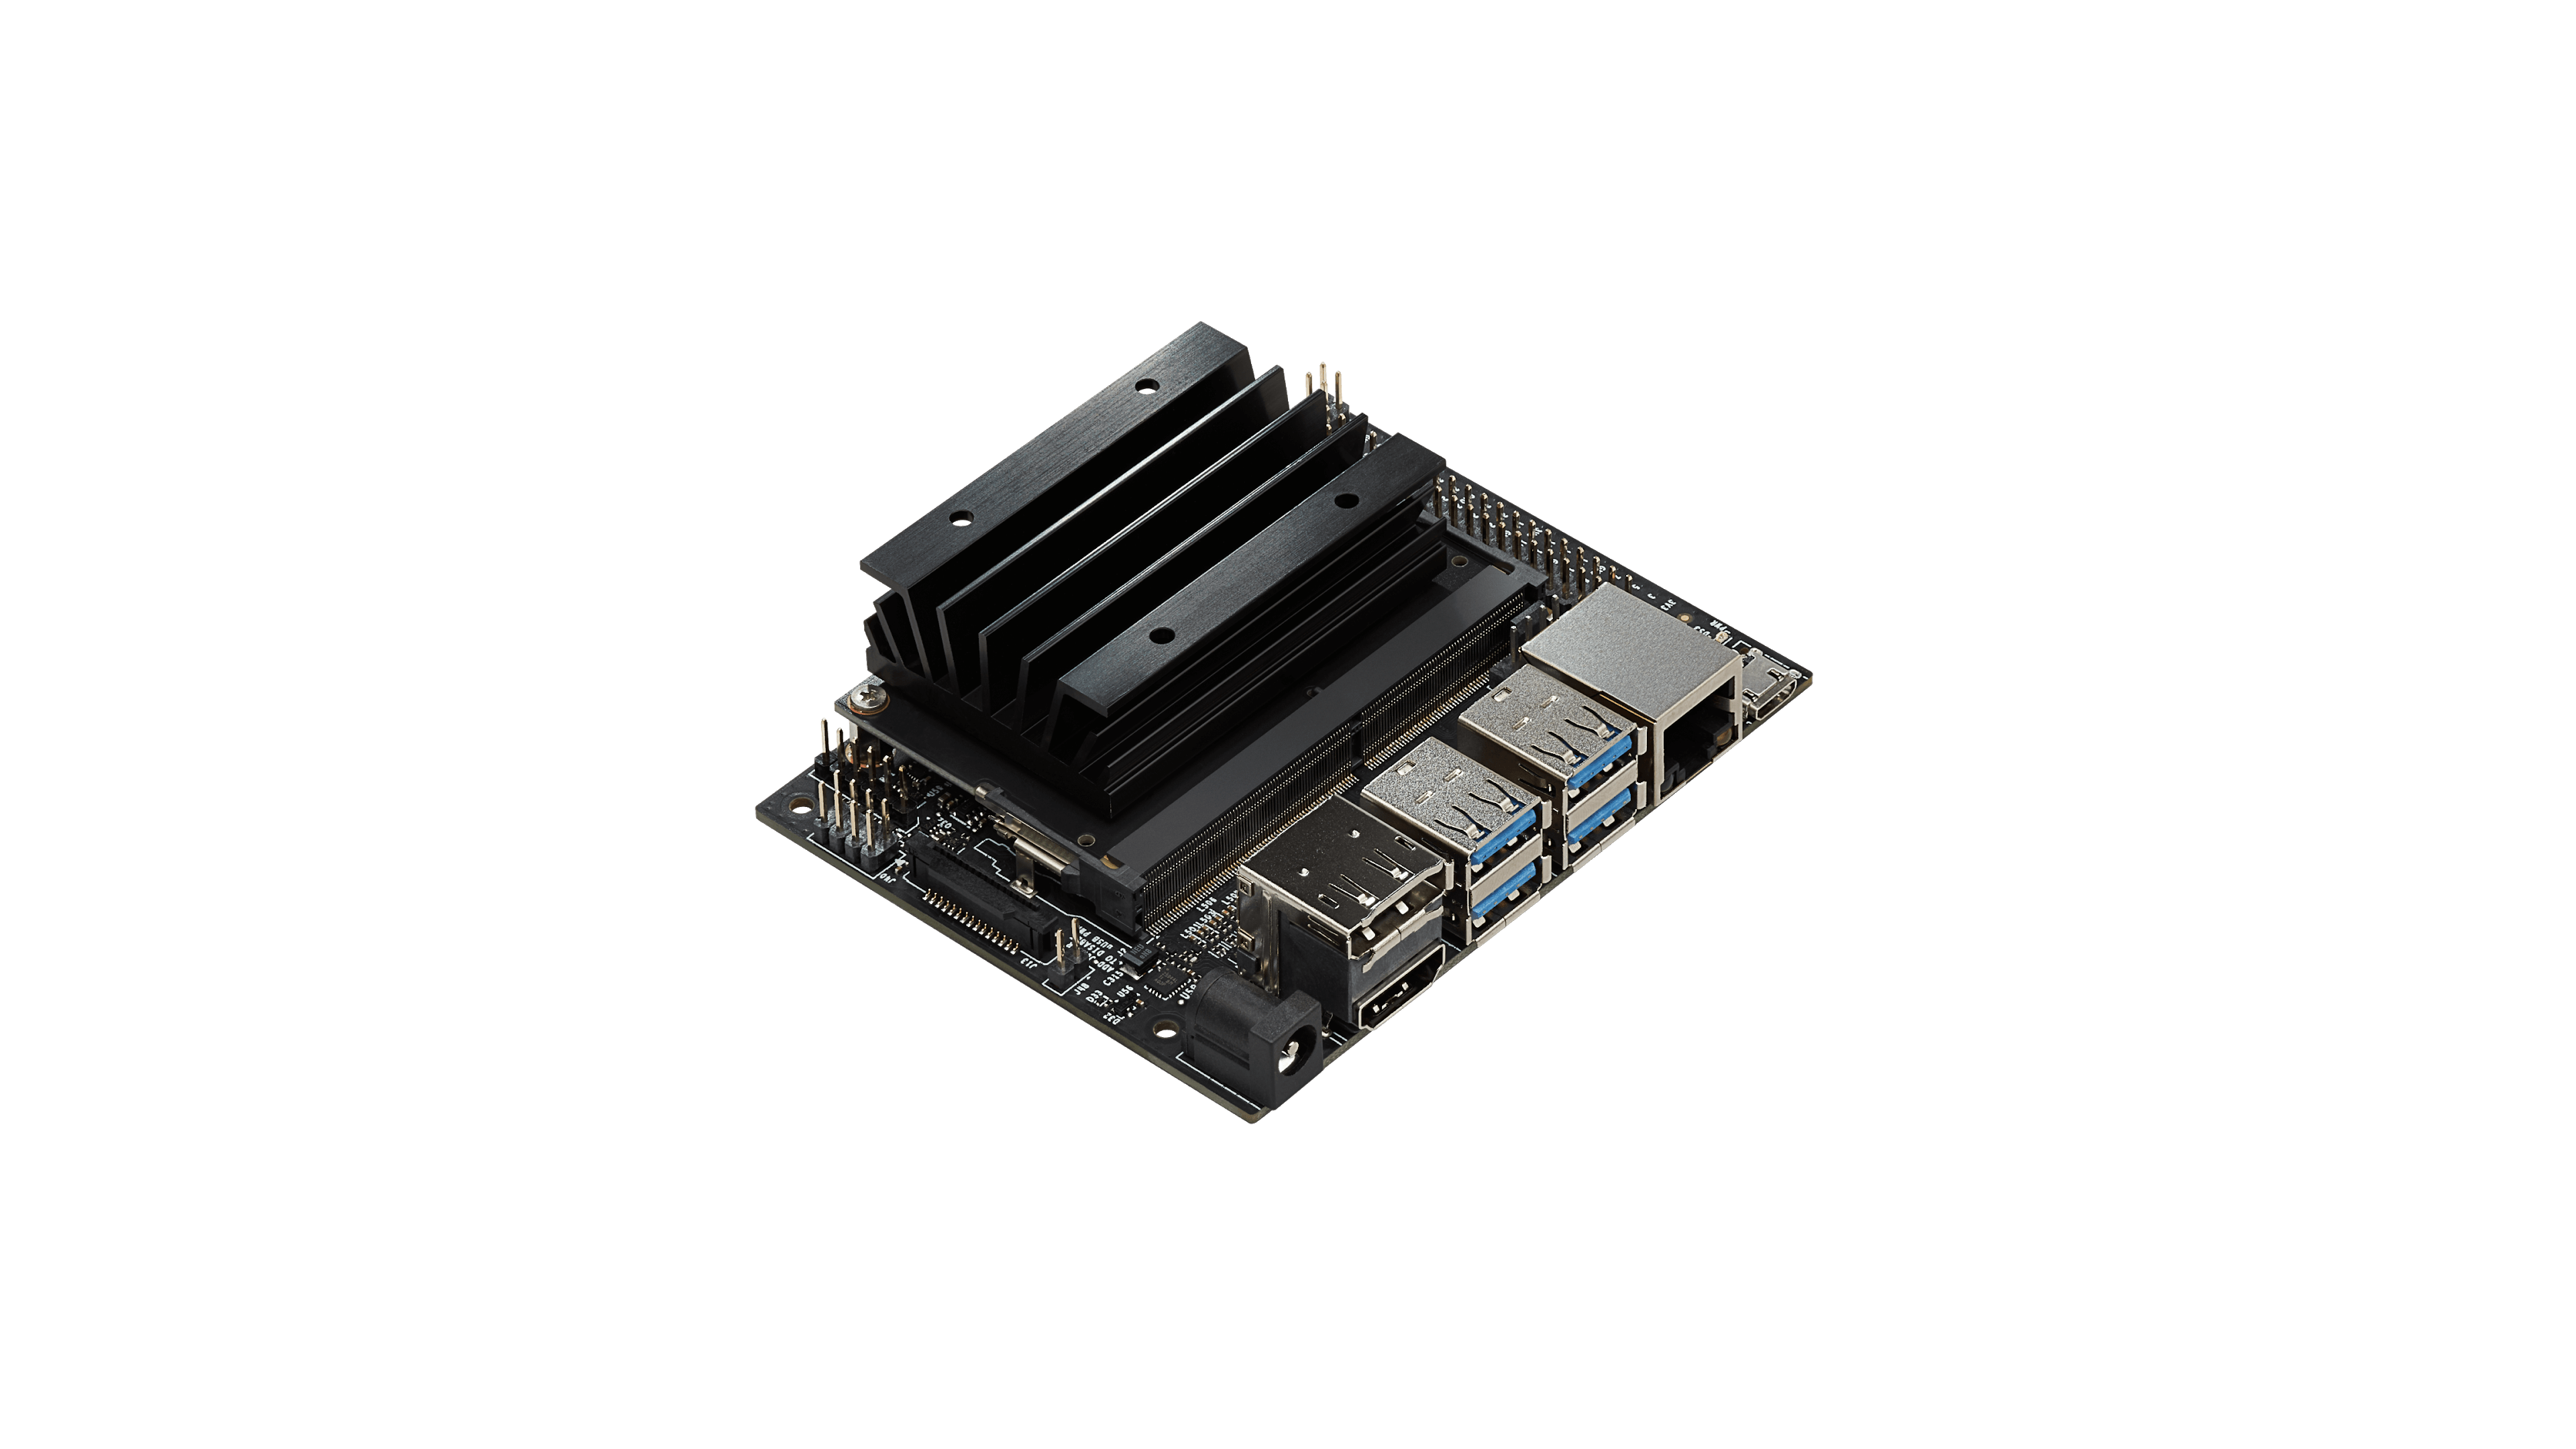
\includegraphics[width=0.4\textwidth]{img/jetson-nano.png}
        \caption{Jetson Nano}
        \label{fig:jetson}
    \end{figure}

    \noindent The project has been developed using the C++ programming language and the CUDA library. 
    The CUDA library has been used to exploit the GPU capabilities and to perform the image processing operations in parallel.

    \subsection{Changes} %CAMBIARE TITOLO CHE FA SCHIFO
    The project has been developed in a versioned style. The first version of the project $(v0.5)$ has been developed on January 19th. 
    This version implemented the image processing operations using three different CUDA functions, one for each operation. 
    This operating mechanism slows down the execution time of the program, since the image is copied three times in the GPU memory, and 
    for each operation the image is copied back to the CPU memory, other than the overhead of the CUDA function calls and kernel creation.
    Moreover, this version of the project still implements the black border around the image, which creates a worse looking image when the borders are enlarged.
    In this version, the enlargement of the image must be square, since the complete zooming feature has not been implemented yet.

    The second version of the project $(v0.9)$ has been developed on January 26th. This version encapsulates the three image processing operations in a single CUDA function,
    which is called only once, making the execution faster and reducing the overhead of the CUDA function calls and kernel creation. 
    This version of the project still implements the black border around the image.
    Moreover, this version of the project implements a complete zooming feature, which allows the user to zoom in the image, by selecting a rectangular area of the image.

    The third and final version of the project $(v1)$ has been developed on February 10th. This can be considered the final version of the project, since it implements all the features
    that were planned for the project. This version of the project removes the black border around the image, which makes the image look better when the borders are enlarged, with the technique
    explained in the previous section. 

    The three versions have all been analyzed and compared in terms of execution time and image quality. Moreover, the profiling of the code has been performed to understand the bottlenecks, while 
    also trying to bring the \\% portare al limite l'esecuzione del programma???????
    These results are presented in the following table \ref{tab:expres}.
    % Tabella con i risultati   
    \small
    \begin{table}[ht]
        % \begin{tabular}{|p{1.5cm}|p{4cm}|p{2cm}|p{2.5cm}|p{2.5cm}|}
        \begin{tabular}{|c|c|c|c|}
            \hline
            Version & Global or shared memory& Time to execute & Shared ld/st conflicts \\
            \hline
            v0.5 (19 Jan) & Global & - & /\\
            \hline
            v0.5 (19 Jan) & Shared & - & 0\\
            \hline
            v0.9 (26 Jan) & Global & - & /\\
            \hline
            v0.9 (26 Jan) & Shared & - & 0\\
            \hline
            v1 (10 Feb) & Global & - & /\\
            \hline
            v1 (10 Feb) & Shared & - & 0\\
            \hline
        \end{tabular}
        \caption{Experimental results}
        \label{tab:expres}
    \end{table}

\begin{figure}[h]
    \centering
    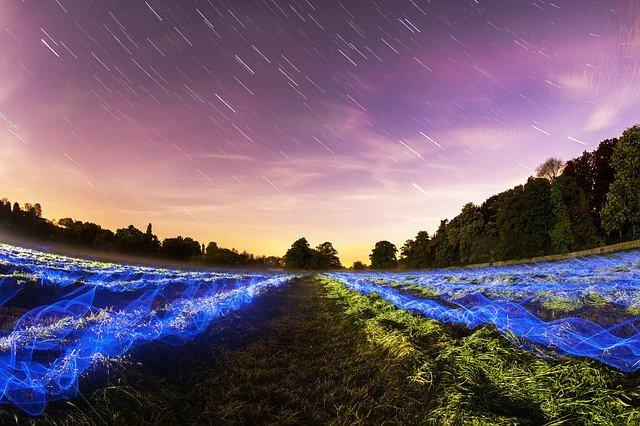
\includegraphics[width=0.5\textwidth]{img/start/sample640x426.jpg}
    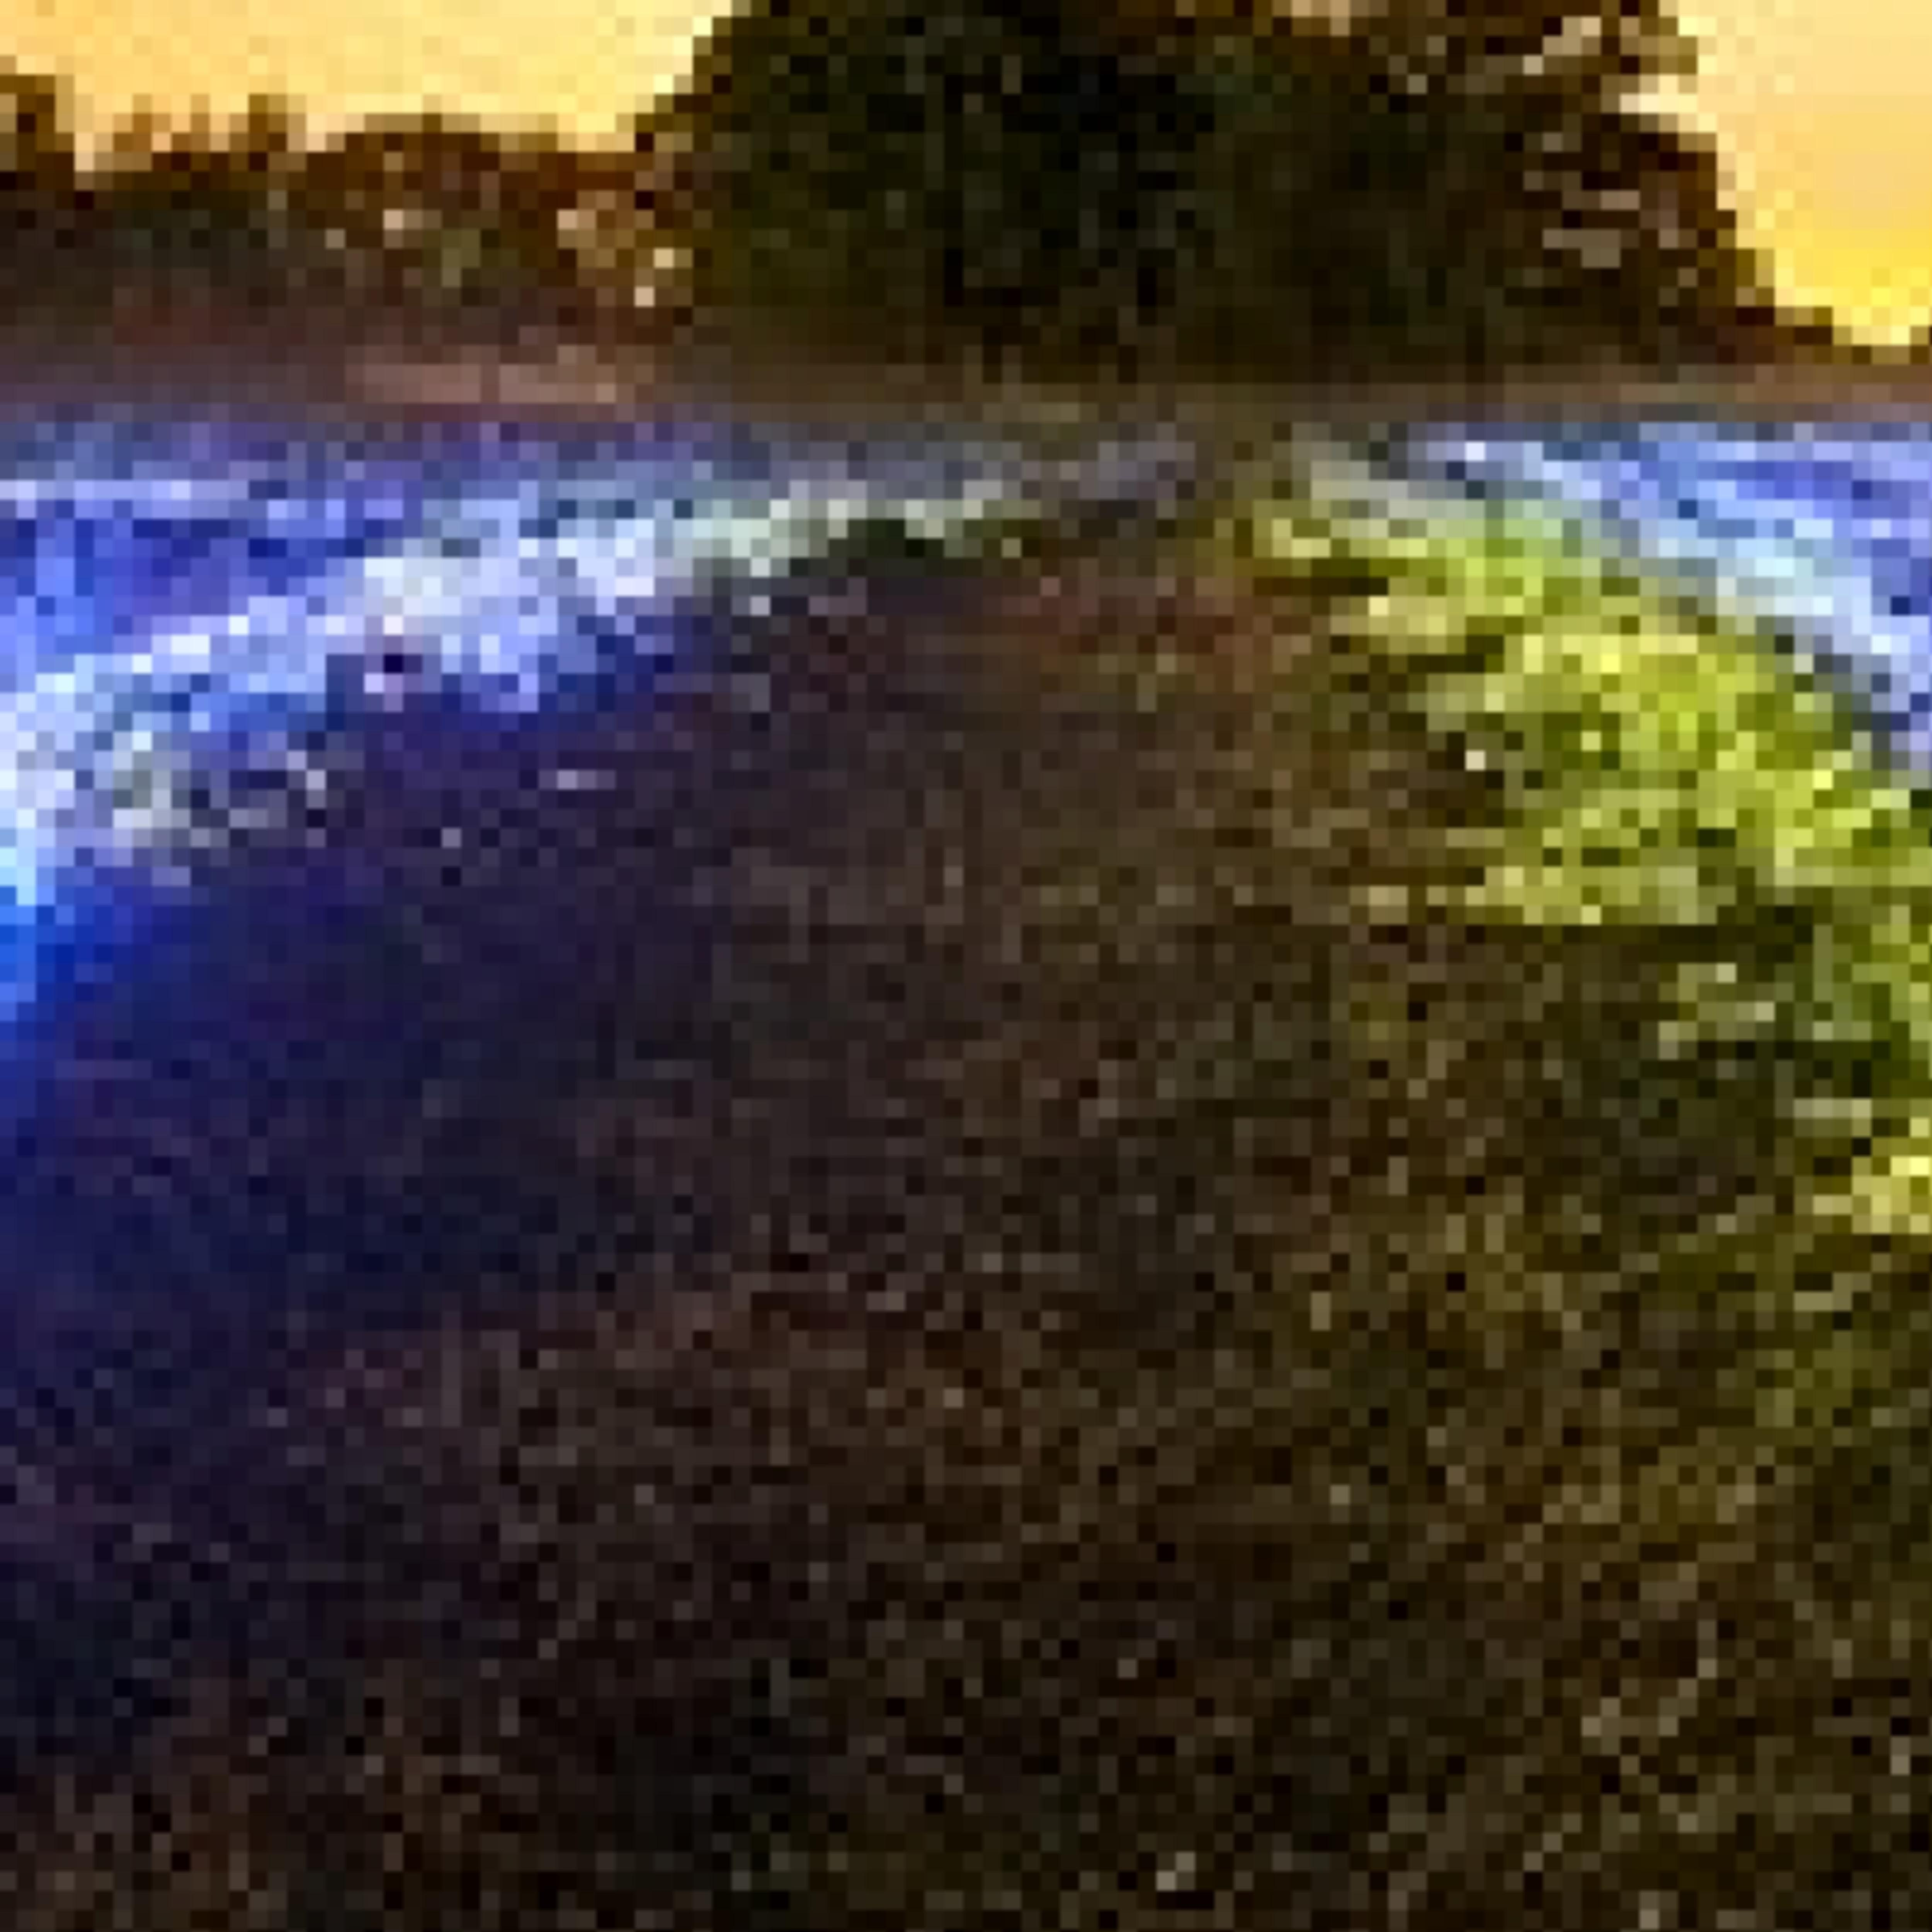
\includegraphics[width=0.3\textwidth]{img/start/selectedZoneCutout.jpg}
    \caption{Original image and zoomed image (v1)}
    \label{fig:original}
\end{figure}